\chapter{信号的采样和采样定理}%
\label{cha:信号的采样和采样定理}

\section{实验目的}%
\label{sec:实验目的\arabic{chapter}}

\begin{enumerate}
	\item 掌握对连续时间信号进行采样的方法,了解采样信号的频谱的特点;
	\item 验证采样定理。
\end{enumerate}

\section{实验原理及方法}%
\label{sec:实验原理及方法\arabic{chapter}}

\begin{enumerate}
	\item 所谓采样信号是对连续时间信号每隔一定的时间抽取一次函数值而组成的一离散时间信号,采样信号$ f_\text{s} $可以表示成连续时间信号$ f(t) $与采样脉冲序列$ p(t) $的乘积,即:

		\begin{align}
			f_\text{s}(t)=f(t)p(t)
		\end{align}

		若采样脉冲序列$ p(t) $是以$ T_\text{s} $为周期的窄脉冲串,称为脉冲采样,$ T_\text{s} $的倒数$ f_\text{s} $为采样频率。$ f_\text{s},f(t),p(t) $的波形如图\ref{fig:矩形脉冲采样信号的频谱}所示:

		\begin{figure}[htpb]
			\centering
			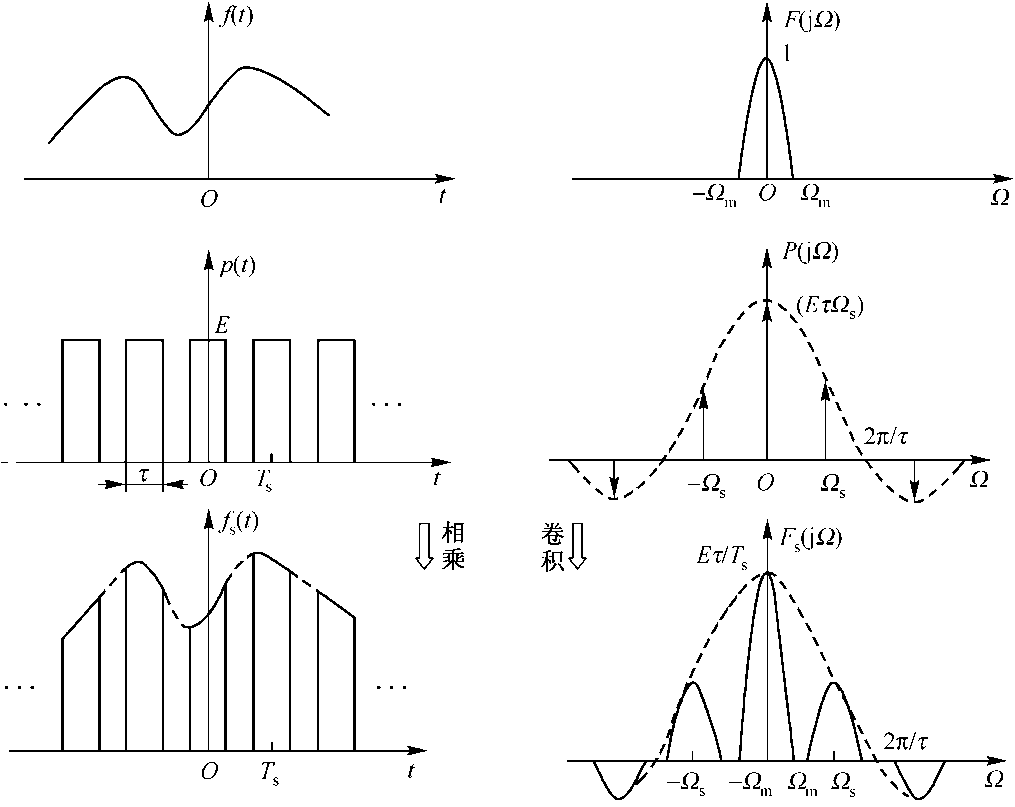
\includegraphics[width=0.8\linewidth]{4-2.png}
			\caption{矩形脉冲采样信号的频谱}
			\label{fig:矩形脉冲采样信号的频谱}
		\end{figure}

		如连续信号的频谱为$ F(\jmath\Omega) $,则采样信号的频谱为$ F_\text{s}(\jmath\Omega) $其波形也见图\ref{fig:矩形脉冲采样信号的频谱}所示:其表达式为:

		\begin{align}
			F_\text{s}(\jmath\Omega)=\sum\limits_{n=-\infty}^{+\infty}P_nF\big(\jmath(\Omega-n\Omega_\text{s})\big)
		\end{align}

		上式表明,采样信号的频谱$ F_\text{s}(\jmath\Omega) $可以看成由采样信号的频谱$ F_\text{s}(\jmath\Omega) $以采样频率$ \Omega_\text{s} $为间隔周期延拓而得到的,在周期延拓过程中幅度被$ P_n $加权。当采样脉冲$ p(t) $是周期矩形脉冲时,采样信号的频谱为:

		\begin{align}
			F_\text{s}(\jmath\Omega)=\dfrac{E\tau}{T}\sum\limits_{n=-\infty}^{+\infty}\text{Sa}(\dfrac{n\Omega\tau}{2})F\big(\jmath(\Omega-n\Omega_\text{s})\big)
		\end{align}

	\item 采样信号在一定的条件下可以恢复出原信号。由采样定理可知,要恢复出原信号首先必须满足$ f_\text{s}>f_\text{m} $,其中$ f_\text{s} $为采样频率,$ f_\text{m} $为原信号的最高频率分量;在此前提下,用一截止频率为$ f_\text{c} $的低通滤波器滤除采样信号中的高频分量则可得到原信号。其中:

		\begin{align}
			f_\text{m}\leqslant f_\text{c}\leqslant f_\text{s}-f_\text{m}
		\end{align}

		当采样频率不满足采样定理,即$ f_\text{s}<2f_\text{m} $时,采样信号的频谱会发生混叠,原信号无法恢复。

		然而,仅包含有限频率的信号极少,而包含较多频率的信号即使在满足采样定理时,恢复后发生失真亦是难免的。
	\item 为了实现对连续信号的采样和采样信号的复原,可以采用图\ref{fig:信号的采样与恢复}的方案。

		\begin{figure}[htpb]
			\centering
			\includegraphics{sample.pdf}
			\caption{信号的采样与恢复}
			\label{fig:信号的采样与恢复}
		\end{figure}

		抗混叠滤波器用来防止原信号频谱过宽而造成采样后信号频谱的混叠,如果实验中采用的信号的频带较窄,则可不用此滤波器;采样器有多种实现电路,本实验中采用运算放大器组成模拟乘法器;重构滤波器为——低通滤波器,可用有源的也可用无源的,本实验中采用简单的$ \pi $型LC低通滤波器,如图\ref{fig:pi 型低通滤波器}所示:

		\begin{figure}[htpb]
			\centering
			\includegraphics{LC.pdf}
			\caption{$ \pi $型低通滤波器}
			\label{fig:pi 型低通滤波器}
		\end{figure}

		其截止频率$ f_\text{c}=\dfrac{1}{\pi\sqrt{LC}} $,标称特性阻抗$ R_\text{ld}=\sqrt{\dfrac{L}{C}} $,若给定$ R_\text{ld} $和$ f_\text{c} $就可按下式计算出元件的数值。

		\begin{align}
			L&=\dfrac{R_\text{ld}}{\pi f_\text{c}}\\
			C&=\dfrac{1}{\pi f_\text{c}R_\text{ld}}
		\end{align}

\end{enumerate}

\section{实验前预习内容}%
\label{sec:实验前预习内容\arabic{chapter}}

\begin{Exercise}
	若连续时间信号是频率为\SI{5}{kHz}的正弦波,采样脉冲$ p(t) $为$ T_\text{s}=\SI{40}{\micro s} $的窄脉冲,试求出采样信号$ f_\text{s}(t) $的频谱。
\end{Exercise}

\langCVfile[Matlab][code:code431.m][Matlab]{code431.m}{src/code431.m}

\begin{figure}[htpb]
	\centering
	%\matlablightfile{MATLAB Command Window}{src/code431.txt}
	\caption{运行界面}
	\label{fig:运行界面code431.m}
\end{figure}

\begin{Exercise}
	设计一$ \pi $型低通滤波器,截止频率为\SI{5}{kHz}, $ R_\text{ld} $为$ \SI{2}{k\ohm} $。
\end{Exercise}

\begin{Exercise}
	若连续时间信号是频率为\SI{1}{kHz}的三角波,估算其有效的频带宽度。该信号经重复频率为$ f_\text{s} $的周期脉冲采样后,若希望通过低通滤波器后的信号失真较小,则采样频率和低通滤波器的截止频率应分别取多少?试设计一满足上述要求的低通滤波器。
\end{Exercise}

\section{实验原理图}%
\label{sec:实验原理图\arabic{chapter}}

\begin{figure}[htpb]
	\centering
	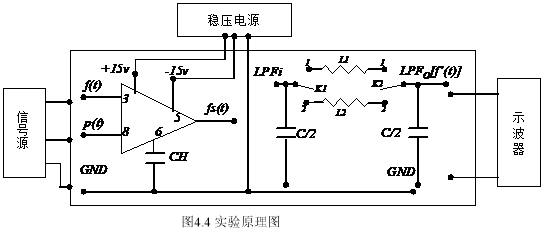
\includegraphics[width=0.8\linewidth]{4-4.png}
	\caption{实验原理图\arabic{chapter}}
	\label{fig:实验原理图\arabic{chapter}}
\end{figure}

\section{实验内容及步骤}%
\label{sec:实验内容及步骤\arabic{chapter}}

\subsection{观察采样信号的波形}%
\label{sub:观察采样信号的波形}

\begin{enumerate}
	\item 将信号源的一路输出调为三角波,频率调为\SI{500}{Hz}作为被采样信号,另一路调为窄脉冲,频率调为\SI{1}{kHz}作为采样脉冲;
	\item 按原理图将两路信号分别加到实验板上的$ f(t) $及$ p(t) $端,用示波器同时观察$ f(t) $和$ f_\text{s}(t) $的波形;
	\item 将窄脉冲的频率(采样频率)改变为\SI{3}{kHz},\SI{6}{kHz}再次观察$ f(t) $和$ f_\text{s}(t) $的波形。
\end{enumerate}

\subsection{验证采样定理与信号恢复}%
\label{sub:验证采样定理与信号恢复}

首先将原理图中的开关K1,K2接1,然后进行下面的操作;

\begin{enumerate}
	\item\label{it:将信号源输出的三角波频率调为1kHz}将信号源输出的三角波频率调为\SI{1}{kHz},采样频率调为\SI{3}{kHz},并将采样信号 接低通滤波器的输入端($ \text{LPF}_\text{i} $), 示波器接低通滤波器的输出端($ \text{LPF}_\text{i} $)端,观察恢复后的波形;
	\item 将采样频率调为\SI{6}{kHz},其它条件不变,观察恢复后的波形;
	\item\label{it:将采样频率调为12kHz}将采样频率调为\SI{12}{kHz},其它条件不变,观察恢复后的波形;
\end{enumerate}

将原理图中的开关K1,K2接2,然后重复\ref{it:将信号源输出的三角波频率调为1kHz}至\ref{it:将采样频率调为12kHz}操作。

\section{实验仪器及设备}%
\label{sec:实验仪器及设备\arabic{chapter}}

双踪示波器一台,函数发生器一台,稳压电源一台,实验板一块。

\section{实验报告要求}%
\label{sec:实验报告要求\arabic{chapter}}

\begin{Exercise}
	绘出实验内容\ref{sub:观察采样信号的波形}中的$ f(t) $和$ f_\text{s}(t) $的波形。
\end{Exercise}

\begin{Exercise}
	绘出实验内容\ref{sub:观察采样信号的波形}中三种不同采样频率下的$ f(t) $和$ f_\text{s}(t) $的波形;比较后得出结论。
\end{Exercise}

\begin{Exercise}
	用Matlab画出对频率为\SI{1}{kHz}的正弦波和频率为\SI{3}{kHz}三角波用采样频率为\SI{6}{kHz}进行理想采样后的时域图和频谱图。
\end{Exercise}

\langCVfile[Matlab][code:code473.m][Matlab]{code473.m}{src/code473.m}

\begin{figure}[htpb]
	\centering
	\matlablightfile{MATLAB Command Window}{src/code473.txt}
	\caption{运行界面}
	\label{fig:运行界面code473.m}
\end{figure}

\begin{figure}[htpb]
	\centering
	\begin{subfigure}[htpb]{.45\linewidth}
		\centering
		%\includegraphics[width=\linewidth]{sine.png}
		\caption{正弦波时域图和频域图}
		\label{fig:正弦波时域图和频域图}
	\end{subfigure}
	\quad
	\begin{subfigure}[htpb]{.45\linewidth}
		\centering
		%\includegraphics[width=\linewidth]{triangle.png}
		\caption{三角波时域图和频域图}
		\label{fig:三角波时域图和频域图}
	\end{subfigure}
	\quad
	\caption{时域图和频域图}
	\label{fig:时域图和频域图}
\end{figure}

